\chapterimage{Week7Safety.png} 
\chapter{Safety}



\begin{table}[H]
\begin{tabular}{| m{1cm} | m{15cm} |}
\hline
\multicolumn{2}{|l|}{\textbf{Expected   Range of Knowledge for Safety}}                                                                          \\ \hline
\multicolumn{2}{|l|}{\textit{Water   Distribution System Operator License Exams}}                                                                                      \\ \hline
D1 & Knowledge of   OSHA/Cal-OSHA safety regulations                                                                                   \\ \hline
D1 & Knowledge of the   components of the Emergency Response Plan                                                                      \\ \hline
D1 & Knowledge of Cal-OSHA   trenching and shoring requirements                                                                        \\ \hline
D1 & Ability to recognize   a confined space                                                                                           \\ \hline
D1 & Knowledge of chemical   handling safety equipment and procedures                                                                  \\ \hline
D1 & Knowledge of confined   space safety equipment and procedures                                                                     \\ \hline
D1 & Knowledge of   electrical safety equipment and procedures                                                                         \\ \hline
D1 & Knowledge of fire   safety equipment and procedures                                                                               \\ \hline
D1 & Knowledge of   hazardous material safety equipment and handling                                                                   \\ \hline
D1 & Knowledge of personal   safety equipment and procedures                                                                           \\ \hline
D1 & Knowledge of safety   regulation requirements (e.g. IIPP)                                                                         \\ \hline
D1 & Knowledge of the   elements of a safety program (e.g. policy statement, training, promotion,   accident investigation, reporting) \\ \hline
D1 & Knowledge of traffic   control procedures                                                                                         \\ \hline
D1 & Knowledge of   trenching safety equipment and procedures                                                                          \\ \hline
D1 & Knowledge of safety   equipment requirements                                                                                      \\ \hline
D3 & Knowledge of   recordkeeping/reporting requirements to OSHA                                                                       \\ \hline
D4 & Ability to develop and implement a safety   plan                                                                                  \\ \hline
\end{tabular}
\end{table}

\newpage



\begin{table}[H]
\begin{tabular}{| m{1cm} |m{15cm} |}
\hline
\multicolumn{2}{|l|}{\textbf{Expected   Range of Knowledge for Safety}}                                                                      \\ \hline
\multicolumn{2}{|l|}{\textit{Water   Treatment Operator License Exams }}                                                                  \\ \hline
T1 & Ability to   demonstrate safe work habits                                                                                         \\ \hline
T1 & Ability to identify   potential safety hazards                                                                                    \\ \hline
T1 & Ability to recognize   unsafe working conditions                                                                                  \\ \hline
T1 & Ability to select and   utilize safety equipment                                                                                  \\ \hline
T1 & Knowledge of   compressed gas safety procedures                                                                                   \\ \hline
T1 & Knowledge of confined   space safety procedures                                                                                   \\ \hline
T1 & Knowledge of   electrical safety                                                                                                  \\ \hline
T1 & Knowledge of   hazardous chemical handling                                                                                        \\ \hline
T1 & Knowledge of   incompatible chemicals                                                                                             \\ \hline
T1 & Knowledge of   lock-out/tag-out procedures                                                                                        \\ \hline
T1 & Knowledge of Material   Safety Data (MSD) sheets                                                                                  \\ \hline
T1 & Knowledge of personal   protective equipment (PPE)                                                                                \\ \hline
T1 & Knowledge of proper   chemical handling techniques                                                                                \\ \hline
T1 & Knowledge of safe   working practices                                                                                             \\ \hline
T1 & Knowledge of the use   of safety equipment                                                                                        \\ \hline
T2 & Knowledge of HAZWOPER   guidelines                                                                                                \\ \hline
T3 & Ability to generate a   written safety plan                                                                                       \\ \hline
\end{tabular}
\end{table}
\newpage


\section{Hazard control approaches}\index{Safety!Hazard control}
\begin{itemize}
\item Treatment plant operators face a variety of workplace safety hazards ranging from physical injuries to hazardous material exposure.  
\item The three principal approaches for hazard control are:
\begin{enumerate}
\item Engineering Controls:  Engineering controls include incorporating safety elements during engineering design and include considerations related to selecting a less hazardous alternatives, establishing  physical barriers and elements related to ventilation.
\item Administrative Controls:  Administrative controls are used to improve safety within the workplace by putting in place policies and rules that reduce the occupational risk faced by workers via altering the way their work is performed.  These include: housekeeping, materials handling and transfer procedures, training, providing facilities to support personal hygiene practices and medical surveillance.
\item Personal Protective Equipment: Personal protective equipment (PPE)\index{Safety!Personal protective equipment (PPE)} is equipment worn to minimize exposure to hazards that cause serious workplace injuries and illnesses.  PPE includes respiratory protection and protective clothing - hard hats, safety
glasses/goggles, work gloves, chemical resistant gloves and safety shoes.

\end{enumerate}
\item The Occupational Safety and Health Administration - OSHA \index{OSHA}, a. Federal Government agency is responsible for establishing and enforcing workplace safety and health regulations.
\end{itemize}


\section{Water treatment hazards}\index{Safety!Water treatment hazards}
\subsection{Hazardous chemicals}\index{Safety!Chemicals}
\begin{itemize}
\item OSHA's Hazardous Waste Operations and Emergency Response (HAZWOPER) \index{HAZPOWER} standards aims to prevent and minimize the possibility of worker injury and illness resulting from potential exposures to hazardous substances.  It requires that employers follow specific work policies, practices, and procedures to protect their workers potentially exposed to hazardous substances.
\item Hazardous chemicals are used throughout water treatment plants and in distribution systems. 
\item To understand the dangers of these chemicals and to take adequate steps OSHA \index{OSHA} requires that the chemical manufacturer, distributor, or importer provide Safety Data Sheets (SDSs) \index{Safety!Safety Data Sheets (SDS)} (formerly MSDSs or Material Safety Data Sheets) for each hazardous chemical to downstream users to communicate information on hazards related to that particular chemical or product.
\item Employers must ensure that the SDSs are available and readily accessible to employees for all hazardous chemicals in their workplace.
\item The SDS includes information such as the properties of each chemical; the physical, health, and environmental health hazards; protective measures; and safety precautions for handling, storing, and transporting the chemical.\\

\end{itemize}


\subsubsection{Effects of Chemical Hazards}\index{Safety!Chemicals!Hazards}

Hazardous chemicals can cause:
\begin{itemize}
\item Headaches, rashes and burns
\item Respiratory problems
\item Lung and liver damage
\item Reproductive damage
\item Cancer
\item Death
\end{itemize} 


\subsubsection{Protection from chemicals}\index{Safety!Chemicals!Protection}
\begin{itemize}
\item NSF/ANSI 61 \index{NSF/ANSI 61 standards} establishes minimum health-effects requirements for the chemical contaminants and impurities that are indirectly imparted to drinking water from products, components and materials used in drinking water systems.
\item NSF/ANSI 61 standards covers specific materials or products that come into contact with drinking water, drinking water treatment chemicals or both. The products and materials covered by the scope of this standard include but aren’t limited to:
\begin{itemize}
\item Protective barrier materials (cements, paints, coatings)
\item Joining and sealing materials (gaskets, adhesives, lubricants)
\item Mechanical devices, including treatment products (water meters, valves, filters)
\item Pipes and related products (pipes, hoses, fittings)
\item Plumbing devices (faucets, drinking fountains)
\item Process media (filter media, ion exchange resins)
\item Nonmetallic potable water materials
\end{itemize}
\item Chemical manufacturers, distributors, or importers are required to provide Safety Data Sheets (SDS) \index{Safety!Safety Data Sheets (SDS)} (formerly MSDSs or Material Safety Data Sheets) for each hazardous chemical to downstream users to communicate information on these hazards.
\begin{itemize}
\item Reading and understanding the associated Safety Data Sheets
\item Wearing appropriate Personal Protective Equipment
\item Implementing safe work practices by:
\begin{itemize}
\item \textbf{NEVER:} Eating, drinking or smoking when working with hazardous chemicals, and washing or storing PPE with personal clothing.
\item \textbf{ALWAYS:}Washing hands, arms and face with soap and water after use, ensuring integrity of PPE before and after use and also very importantly ensuring  readiness to deal with chemical exposure or spill.
\end{itemize}
\end{itemize}
OSHAs SDS Guidance Document in Appendix \ref{appendix:SDS Content - OSHA Guidance} provides detailed information on its structure and contents. A sample SDS is provided in Appendix \ref{appendix:Sample SDS}.
\end{itemize}
\subsubsection{Ensuring chemicals storage compatibility}\index{Safety!Chemicals storage}

Storing incompatible chemicals together could create a hazardous reaction such as the production of toxic gas, accelerated corrosion, or an exothermic reaction - reaction that releases heat, potentially resulting in an explosion and/or fire. 
A table showing chemical compatibility of water treatment related chemicals is provided in Appendix \ref{appendix:Chemical compatibility table}.
\begin{table}[H]
\begin{tabular}{|m{7cm}|m{7cm}|}
\hline
\multicolumn{1}{|c|}{\textbf{Examples of Incompatible Chemicals}}                        & \multicolumn{1}{c|}{\textbf{Hazardous Reactions}} \\ \hline
Powdered activated carbon (PAC) \index{Powdered activated carbon (PAC)}, an adsorption powder, should not be mixed with potassium
permanganate, an oxidizing powder                                                            & Excessive heat generation, with the possibility of
explosion and fire. Note: PAC alone is extremely
combustible 
 \\ \hline
Calcium hypochlorite (HTH), a combination base/oxidizer
should not be exposed to moisture or mixed with
viscous fluid such as oil. & Excessive heat, fire or explosion possible and may
provide an ignition source for combustible materials.
            \\ \hline
Calcium oxide, a strong base available only as a
powder, should not be exposed to moisture & Excessive heat, fire which may provide an ignition source for combustible materials.
 \\ \hline
Calcium oxide cannot be stored with alum & Water of hydration in alum will react with quicklime releasing excessive heat and causing an explosion.
 \\ \hline
\end{tabular}
\caption{Examples of incompatible chemicals}
\label{table:Incompatiblechemicals}
\end{table}

\subsection{Falls}\index{Safety!Falls}
\begin{itemize}
\item Falls are one of the leading causes of injuries and deaths on the job. 
\item Fall protection is a combination of methods and devices used to protect workers from falling off, onto, or through working levels.
\item Working on top of tanks, walkways roofs, and other elevated surfaces more than 4 feet or when working above open tanks or hazardous machinery requires the provision of fall protection.
\item Fall protection methods and devices are typically divided into two categories: 
\begin{itemize}
\item those that prevent falls, and
\item those that arrest falls.
\end{itemize}
\item Examples of fall prevention devices include: rails, guards, guardrails, barriers.  Fall-arrest systems include: safety nets and hole covers.
\item To prevent employees from being injured from falls, OSHA requires employers to provide:
\begin{itemize}
\item Guard every floor hole into which a worker can accidentally walk (using a railing and toe-board or a floor hole cover).
\item A guard rail and toe-board around every elevated open sided platform, floor or runway.
\item Regardless of height, if a worker can fall into or onto dangerous machines or equipment (such as a vat of acid or a conveyor belt) employers must provide guardrails and toe-boards to prevent workers from falling and getting injured.
\item Other means of fall protection that may be required on certain jobs include safety harness and line, safety nets, stair railings and hand rails.
\end{itemize}
\end{itemize}
\begin{center}
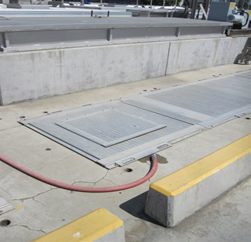
\includegraphics[scale=0.8]{SafetyFallProtection1}\hspace{1cm} 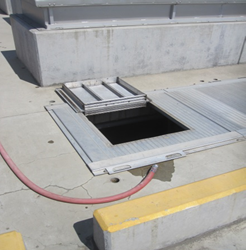
\includegraphics[scale=0.8]{SafetyFallProtection2}\\
\end{center}
\subsection{Noise}\index{Safety!Noise}
\begin{itemize}
\item Noise as a hazard is sound that is especially loud or impacting. 
\item A water treatment plant has equipment that produces high noise levels both continuously and intermittently. 
\item As such, it is important to be aware of this hazard and to take preventive steps to reduce exposure to damaging noise levels by wearing effective hearing protection and to minimize the duration of the exposure to the noise.
\item OSHA's permissible exposure limit (PEL) is 90 dBA for all workers for an 8 hour day.
\end{itemize}

\subsection{Electrical hazards}\index{Safety!Electrical hazards}
\begin{itemize}
\item The main hazards of working with electricity are: 
\begin{itemize}
\item Electric shock and burns from contact with live parts.
\item Injury from exposure to electrical arcing (when electricity jumps from one circuit to another) fire.
\end{itemize}
\item Ordinary 120V electricity can be fatal; most water facility electrical systems operate at 120 to 400V or more.  
\item All voltages should be considered dangerous and potentially life threatening.  
\item Safe working rules and practices that should be followed when working on electrical systems
\item Before working on an electrical system, perform a job hazard analysis to determine any potential hazards and methods of abating those hazards.
\end{itemize}

\subsection{Trenching \& excavation hazards}\index{Safety!Trenching \& excavation}
\begin{itemize}
\item Trench collapses, or cave-ins, pose the greatest risk to workers’ lives.
\item Potential hazards related to trenching include: falls, falling loads, hazardous atmospheres, and incidents involving mobile equipment including vehicular traffic.
\item OSHA \index{OSHA} standards require, before any worker entry, that employers have a competent person
inspect trenches daily and as conditions change to ensure elimination of excavation hazards. 
\item Key elements related to ensuring trench safety \index{Trench safety}:
\begin{enumerate}
\item Ensure that there's a safe way to enter and exit.
\begin{itemize}
\item Ramps for access/egress must be designed by a competent person and be capable of handling the intended loads.
\item A stairway, ladder or ramp must be provided within 25 lateral feet of employees in trench excavations greater than 4 feet.
\item Ladders should extend a minimum distance of 3 feet past the edge they rest against but not more than 4 feet. 
\end{itemize}
\item Test for atmospheric hazards such as low oxygen, hazardous fumes and toxic gases when > 4 feet deep.  
\item If the environment has the potential for a hardous atmosphere, adequate precautions need to be taken to prevent worker exposure to those conditions.
\item Inspect trenches at the start of each shift and following a rainstorm or
other water intrusion.
\item Keep excavated soil (spoils) \index{Spoils}and other materials at least 2 feet from trench edges. If materials need to be closer than two feet from the edge of the trench, install an effective barrier to prevent them from falling into the excavation.
\item Ensure trenches have cave-in protection.
\begin{itemize}
\item Trenches 5 feet deep or greater require a protective system unless the excavation is made entirely in stable rock.
\item Trenches 20 feet deep or greater require that the protective system be designed by a registered professional engineer.
\item Types of protective systems \index{Safety!Trenching \& excavation!Protective systems}:
\begin{itemize}
\item \textbf{Benching} \index{Safety!Trenching \& excavation!Protective systems!Benching} - excavating the sides of an excavation to form one or a series of horizontal levels or steps.
\item \textbf{Sloping} \index{Safety!Trenching \& excavation!Protective systems!Sloping} - involves cutting back the trench wall at an angle inclined away from the excavation.  A good rule of thumb is to slope the sides of the excavation to an angle not steeper
than 1½:1 (for every foot of depth, the trench must be excavated back 1½ feet). A slope of this gradation is safe for any type of soil.
\begin{figure}[H]
\begin{center}
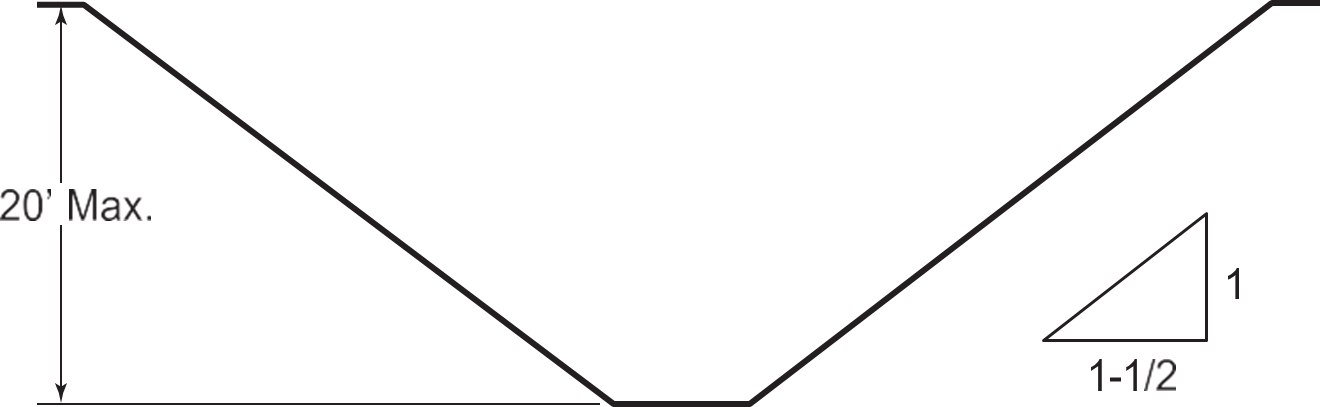
\includegraphics[scale=0.6]{TrenchSlope}\index{Safety!Trench slope}
\caption{Trench slope}
\end{center}
\end{figure}
\item \textbf{Sheeting} \index{Safety!Trenching \& excavation!Protective systems!Sheeting} - wooden sheets or metal plates are placed against the side of the trench or excavation to hold back the walls. Uprights placed vertically along the face of the trench wall are used to support the sheeting. Stringers or wales are placed horizontally along the uprights in which trench braces are attached to prevent cave-in.  It is most often used in shallow excavations or trenches where there is a risk of soil collapse but where the pressures are not excessively high.
\item \textbf{Shoring} \index{Safety!Trenching \& excavation!Protective systems!Shoring} - requires installing aluminum hydraulic or other types of supports designed to support the walls of a trench. Shoring is essential in deeper excavations or in situations where the excavation walls are unstable or subject to higher pressures. It is also crucial when working near existing structures or in urban environments where the stability of adjacent buildings is a concern.
\item \textbf{Shielding} \index{Safety!Trenching \& excavation!Protective systems!Shielding} -  uses a two-sided, braced box sometimes referred to as a drag shield or trench box, which is open at the top, bottom and ends.
\end{itemize}
\begin{figure}[H]
\begin{center}
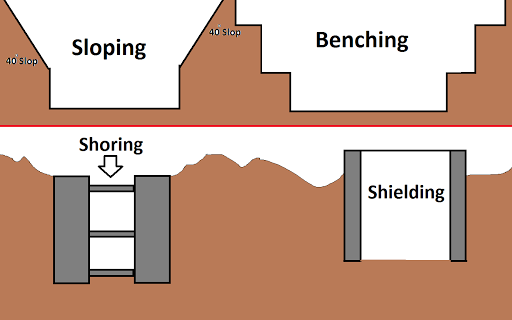
\includegraphics[scale=0.6]{TrenchProtection}
\caption{Trench protection systems}
\end{center}
\end{figure}
\end{itemize}
\end{enumerate}
\end{itemize}
\subsection{Rotating and moving equipment}\index{Rotating and moving equipment}

\begin{itemize}
\item All rotating and moving equipment should be guarded. 
\item The best method for preventing machinery-related injuries is through use of equipment guards enforced through engineering and administrative controls.   
\item The best way to prevent this type of injury is to install point-of-operation guards that prevent contact with nip points, pinch points, rotating parts, flying chips, and sparks.
\end{itemize}
\begin{center}
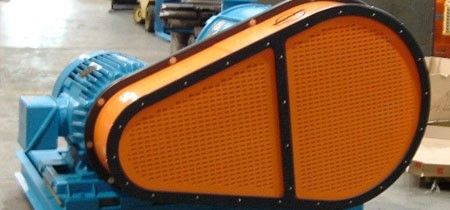
\includegraphics[scale=0.6]{SafetyMachineGuarding}\index{Safety!Machine guarding}\\
\end{center}

\subsection{Heat stress}\index{Safety!Heat stress}
\begin{itemize}
\item Heat stress falls into two categories: heat illness and heat stroke. 
\item Both are serious conditions and should not be taken lightly. 
\item Heat stress can result from: 
\begin{itemize}
\item High temperature and humidity, dehydration from low fluid consumption
\item Direct sun exposure (with no shade) or extreme heat, 
\item Limited air movement (no breeze or wind), 
\item Physical exertion, Use of bulky protective clothing and equipment, 
\item Poor physical condition or ongoing health problems, 
\item Some medications
\item Pregnancy
\end{itemize}
\item Under OSHA regulations, employers are obligated to provide a workplace free of conditions or activities that either the employer or industry recognizes as hazardous and that cause, or are likely to cause, death or serious physical harm to employees when there is a feasible method to abate the hazard. This includes heat-related hazards that are likely to cause death or serious bodily harm.
\item NIOSH \index{National Institute for Occupational Safety and Health (NIOSH)} has published recommendations for employers about how to prevent heat-related illnesses.
\item California's Heat Illness Prevention Standard requires employers to provide training, water, shade, and planning. A temperature of 80°F triggers the requirements. 
\end{itemize} 

\subsection{Fire safety}\index{Safety!Fire safety}
\begin{itemize}
\item Fires are classified based upon the material involved in the fire - Table \ref{table:FireClassification}.  
\item It is very important to note that the fire fighting measures are specific to the material involved and if these measures are not followed, it may aggravate the situation or pose additional safety hazards.
\item Many gasses are explosive when present in certain ratios with oxygen. These ratios are defined by the upper explosive limit(UEL) and the lower explosive limit (LEL). 
\item The minimum concentration of a particular combustible gas or vapor necessary to support its combustion in air is defined as the Lower Explosive Limit (LEL) \index{Safety!Lower explosive limit (LEL)} for that gas. Below this level, the mixture is too “lean” to burn. 
\item The maximum concentration of a gas or vapor that will burn in air is defined as the Upper Explosive Limit (UEL) \index{Safety!Upper explosive limit (UEL)}. Above this level, the mixture is too “rich” to burn.
\item The range between the LEL and UEL is known as the flammable range for that gas or vapor.\\
For example: Methane has an LEL of 5\% and a UEL of 15\% and thus its flammable range is between 5\% and 15\% concentration levels.
\end{itemize}
\begin{table}[h!]
\begin{tabular}{|C{2cm}|p{5.5cm}|p{5.5cm}|}
\hline
%\multicolumn{1}{|c|}{\textbf{CLASSIFICATION}} & \multicolumn{1}{c|}{\textbf{MATERIAL INVOLVED}}                                                                                                                                                                                                                                             & \multicolumn{1}{c|}{\textbf{METHODS FOR EXTINGUISHING \\SMALL   FIRES}}                                                                                                                                                                                       \\ \hline
\multicolumn{1}{|c|}{ \textbf{CLASS}} & \multicolumn{1}{c|}{ \textbf{MATERIAL INVOLVED}} & \multicolumn{1}{c|}{ \textbf{MEASURES TO FIGHT SMALL FIRES} }\\ \hline

CLASS A                                       & This class of fire involves ordinary combustibles  or fibrous material, such as wood, paper, cloth, paper, and some plastics.                                                                                                                                                               & Extinguish with pressurized   water, foam, or multipurpose dry chemical extinguishers. Do not use carbon   dioxide or ordinary dry chemical extinguishers on Class A fires.                                                                                \\ \hline
CLASS B                                       & Class B fire is flammable or   combustible liquids such as gasoline, diesel, kerosene, paint, paint   thinners, and propane.                                                                                                                                                                & Extinguish Class B fires by   removing oxygen, by preventing vapors from reaching ignition sources, or by   inhibiting the chemical chain reaction. Use foam, carbon dioxide, ordinary   dry chemical, multipurpose dry chemical, and halon extinguishers. \\ \hline
CLASS C                                       & A Class C fire is energized   electrical equipment, such as motors, motor controls, switches panel boxes,   and power tools.                                                                                                                                                                & Extinguish Class C fires by   using carbon dioxide, ordinary dry chemical, multipurpose dry chemical, and   halon-free extinguishers.                                                                                                                      \\ \hline
CLASS D                                       & A Class D fire is certain   combustible metals, such as magnesium, titanium, potassium, and sodium. These   metals burn at high temperatures and give off sufficient oxygen to support   combustion. They may react violently with water or other chemicals and must be   handled with care. & Extinguish Class D fires by   using dry powder extinguishers made especially for this type of fire                                                                                                                                                         \\ \hline
\end{tabular}
\caption{Fires classifications}\index{Safety!Fire safety!Fire Classifications}
\label{table:FireClassification}
\end{table}

\section{Safety practices}\index{Safety practices}


\subsection{Lockout-Tagout (LOTO)}\index{Safety!Lockout-Tagout (LOTO)}
\begin{itemize}
\item When conducting routine inspections, repairs and maintenance activities, requires meeting the mandates of OSHAs Lock-Out/Tag-Out (LOTO) program.
\item The LOTO program is designed to prevent injury or fatalities.  
\item It involves preventing an equipment from accidentally starting up and release of all stored energy. 
\item Hazardous energy \index{Safety!Hazardous energy} sources include: 
\begin{itemize}
\item Electrical 
\item Mechanical
\item Hydraulic
\item Pneumatic 
\item Chemical 
\item Thermal  
\item Other energy
\end{itemize}
\item LOTO involves established and documented procedures specific to an equipment or machinery.
\item LOTO typically comprises of:\\
\begin{itemize}
\item Notifying affected employees
\item Stopping and isolating the equipment
\item Releasing stored energy
\item Verification of the isolation and de-energization
\item Placing lock-out devices which use a positive means such as a lock, either key or combination type, to hold an energy isolating device in the safe position and prevent the energizing of a machine or equipment
\item Appropriately tagging the devices to indicate its non-operation and that it may not be operated until the tagout device is removed
\end{itemize}
\end{itemize}
\subsection{Personal protective equipment (PPE)}\index{Safety!Personal protective equipment (PPE)}
\begin{itemize}
\item Employees depend on PPE to protect themselves from hazards and perform daily duties. 
\item PPE includes but is not limited to safety glasses, face shields, hard hats, gloves, foot protection, and durable and disposable chemical-protective clothing. 
\item Respirators and fall protection might also be required.
\item Respirators and fall protection fall under separate OSHA \index{OSHA} standards. The National Institute for Occupational Safety and Health (NIOSH)\index{National Institute for Occupational Safety and Health (NIOSH)} is responsible for testing and approving respirators and providing guidance for their use in occupational settings.\\
\end{itemize}
\subsection{Confined space entry}\index{\index{Safety!Confined space entry}Confined space}
\begin{itemize}
\item OSHA defines a confined space as an area that:
\begin{itemize} 
\item is large enough and so configured that an employee's body can enter and perform assigned work
\item has limited or restricted means for entry or exit; and
\item is not designed for continuous employee occupancy.
\end{itemize}
\item A confined space can be either a permit-required confined space or a non-permit required confined space.
\item A \textbf{permit-required confined space} \index{Permit-required confined space} is one which has one or more of the following characteristics:
\begin{itemize}
\item Contains (or has the potential to contain) a hazardous atmosphere,
\item Contains a material that has the potential for engulfment of an entrant,
\item Has an internal configuration such that an entrant could be trapped or asphyxiated by inwardly converging walls or by a floor which slopes downward and tapers to a smaller cross-section, OR
\item Contains any other recognized serious safety or health hazard.
\end{itemize}
\item A \textbf{non-permit confined space} \index{Non-permit confined space} is defined as a confined space that does not contain any hazard capable of causing death or serious physical harm.
\item At a permit-required confined space where entry is planned, the entry supervisor - person responsible for determining if acceptable entry conditions are present  authorizes entry and oversees entry operations, and for terminating entry as required by this section.
\item Following is required for each each confined space entry:
\begin{enumerate}
\item Evaluate the confined space for hazards including:
\begin{itemize}
\item Atmospheric hazards:
begin{itemize}
\item Flammable gas, vapor, or mist
\item Airborne combustible dust
\item Oxygen concentration below 19.5\% or above 23.5\%
\item Hazardous substances 
\item Engulfment hazards 
\end{itemize}
\item Get a permit, if necessary.
\item Inform employees of the risk
\item Implement safety controls
\item Provide training to each affected employee before they begin their duties.
\end{enumerate}
\end{itemize}
\subsection{Material handling ergonomics}\index{Safety!Material handling ergonomics}
\begin{itemize}
\item Water operators are potentially subject to risk of musculoskeletal injuries associated with handling heavy or unwieldy objects including tools and supplies as part of their daily work routine.
\item The risk and severity of these injuries can be mitigated through utilizing proper ergonomic techniques which include:
\begin{itemize}
\item Use mechanical means (e.g. hand trucks, pushcarts, etc.) when possible for heavier or awkward loads.
\item It is easier and safer to push than to pull.
\item Keep loads as close to the body as possible and do not twist while lifting, carrying, or setting down a load. Nose, shoulders, hips, and toes should all be facing the same direction.
\item Minimize reaching.
\item As a general rule, bend at the knees, not the hips.
\item Get help when needed. Do not lift or carry things you don’t feel comfortable with, no matter how light the load.
\item Plan ahead for all parts of the lift: lifting, carrying, and setting down.
\item Use personal protective equipment where needed, such as gloves with good grip and steel-toed boots where appropriate.
\item Implement rest breaks and job rotation for frequent and/or heavy lifting.
\end{itemize}
\end{itemize}